\subsection{Decision}
The first step was to recognize if the decision of Dean is positive or negative.
The conversion was made according to table~\ref{table:positive_negative}.
A new column of type boolean was created which indicates whether decision is positive or negative.
It turned out that the most numerous group of answers from the dean's office is status closed from unkown reasons as it is visible on Fig.~\ref{fig:application_status_countplot}. The dataset with decision column was very unbalanced what can be seen Fig.~\ref{fig:decision_countplot}. The balanced dataset was needed so the number of positive was reduced to the negative decision quantity. This resulted in a balanced set of decisions as in Fig~\ref{fig:balanced_decision_countplot}.

\begin{figure}
    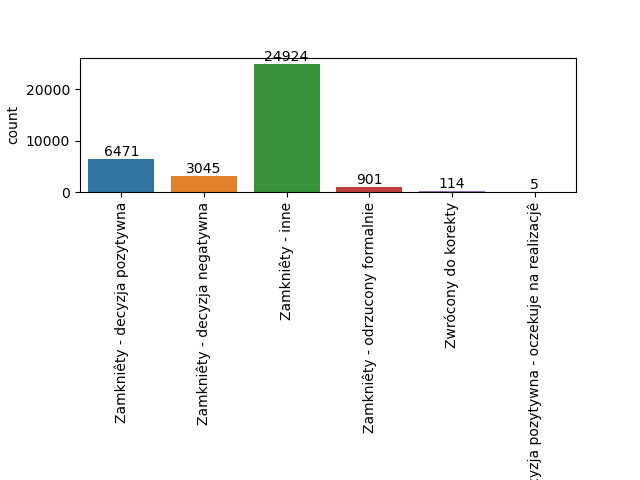
\includegraphics[width=0.5\textwidth]{img/application_status_countplot.png}
    \caption{Application status countplot}
    \label{fig:application_status_countplot}
\end{figure}

\begin{figure}
    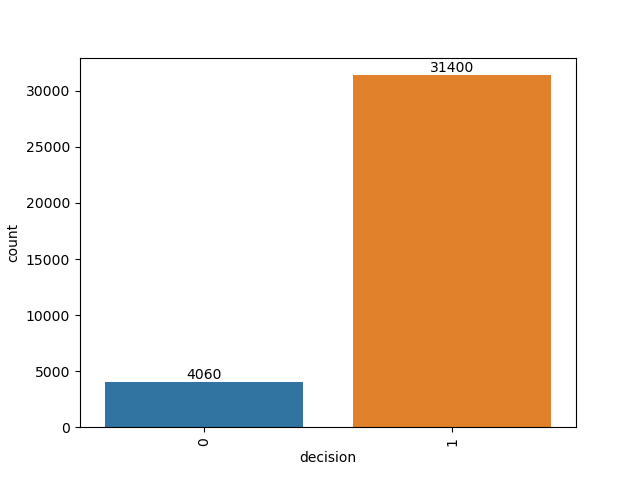
\includegraphics[width=0.5\textwidth]{img/decision_countplot.png}
    \caption{Decision countplot}
    \label{fig:decision_countplot}
\end{figure}

\begin{figure}
    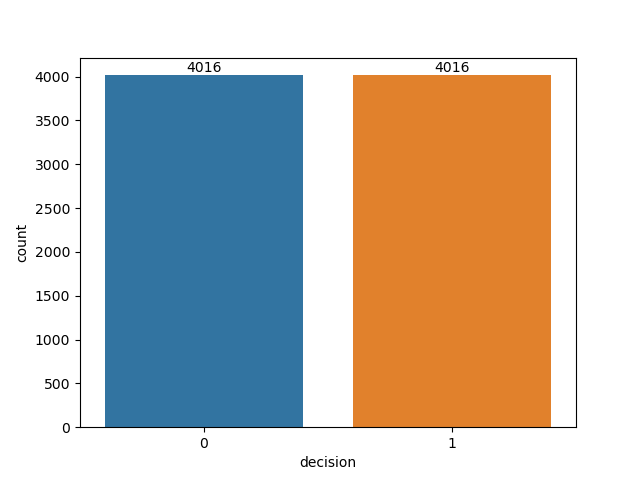
\includegraphics[width=0.5\textwidth]{img/balanced_decision_countplot.png}
    \caption{Balanced decision countplot}
    \label{fig:balanced_decision_countplot}
\end{figure}

\begin{table}
    \caption{Convert status into dean's decision.}
    \label{table:positive_negative}
    \begin{tabular}{|p{0.2\textwidth}|p{0.2\textwidth}|}
        \hline
            \textbf{positive} & \textbf{negative} \\
        \hline
            Zamkniety - decyzja pozytywna & Zamkniety - decyzja negatywna \\ 
        \hline
            Zamkniety - inne & Zamkniety - odrzucony formalnie \\
        \hline
            Decyzja pozytywna - oczekuje na realizacje & Zwrócony do korekty \\
        \hline
        
    \end{tabular}
    
\end{table}


\subsection{Data transformation}
At first columns which definitely should not be significant were removed. For example 'student' column was marked as not significant. The decision should not be performed according to ID of the person. All columns which should be significant was converted into numerical representation.
There was 42 columns in dataset. Only a few of them were numerical. Other were categorical. Using \textit{pd.factorize()} method unique values from each columns were extracted and converted into categorical codes.
There was two columns that were marked as significant, but were not converted into numberical representation due to complexity of the solutions. One of those was 'Level of thesis progress' which was not structured sentences with description about level of the thesis. The decision was made not to sink into this trying to convert it. The second column was 'Missing subjects codes' which had a form of `['A,B,C','C,D']` where letters were subject codes.
